\documentclass[10pt,a4paper]{report}
\usepackage[utf8]{inputenc}
\usepackage{amsmath}
\usepackage{amsfonts}
\usepackage{amssymb}
\usepackage{rotating}
\setlength{\parindent}{0pt}
\usepackage{booktabs}
\title{Relazione Test Multitraccia}
\author{Luca Flammia}
\begin{document}
\maketitle
%\begin{sidewaystable}
%\section*{Tabelle Studiate}
%\begin{tabular}{@{}lllllllllllllllll@{}}
%\label{RIGHE}
%\toprule
%ID\_DICHIARAZIONE & a\_anno & a\_mese & a\_trimestre & a\_imponibile & a\_peso & a\_quantita & a\_codice\_listino & a\_raggruppamento & a\_um\_codice & a\_descrizione & a\_cod\_categoria & a\_cod\_sottocategoria & a\_cod\_tipologia & a\_cod\_sottotipologia & a\_cod\_comparto & ID\_VOCE \\ \midrule
%....              & ....    & ....    & ....         & ....          & ....    & ....        & ....               & ....              & ....          & ....           & ....              & ....                   & ....              & ....                   & ....             & ....     \\ \bottomrule
%\end{tabular}
%\end{sidewaystable}
%\newpage
\section*{Analisi preliminare}
Alcune informazioni sono state estratte partendo dai dati in formato CSV delle relative tabelle considerate. Mediante l'uso del linguaggio Python, sono stati analizzati i dati attraverso l'ausilio delle opportune librerie ovvero
\begin{itemize}
\item \textbf{Pandas} per utilizzo dataframe; 
\item \textbf{Numpy} per calcolo matematico con uso di array;
\item \textbf{Matplotlib} per la visualizzazione dei grafici. 
\end{itemize}
La tabella \underline{RICEVUTE} ha 6273 righe e 8 colonne, ogni riga specifica il 

\textbf{codice\_ordine} del prodotto, identificato univocamente dal valore assegnato nella colonna \textbf{ID\_DICHIARAZIONE}. Nelle colonne \textbf{a\_peso}, \textbf{a\_quantita}, \textbf{a\_imponibile} sono riportati i valori totali per ogni codice ordine, e che sono ricavabili considerando le quantità sommate nelle omonime colonne della tabella \underline{RIGHE} una volta che vengono raggruppate le righe con stesso \textbf{ID\_DICHIARAZIONE}.
La tabella \underline{RIGHE} ha 18116 e 24 colonne: ciò che interessa è saper integrate le informazioni aggiuntive che si hanno in questa tabella con quella precedente.

A questo proposito, si crea una nuova tabella dall'unione delle due (comando SQL $\rightarrow$ INNER JOIN ON ID\_DICHIARAZIONE). Si nota che il codice d'ordine relativo a "ID\_DICHIARAZIONE" = 30154 viene escluso dai dati poiché presente solo nella tabella \underline{RIGHE} ed è costituita da 18115 righe e 20 colonne (si eliminano le colonne doppie). A partire da questi dati, si baserà l'analisi e la creazione del modello predittivo, come riportato nelle pagine seguenti.

%La tabella \textbf{RIGHE} ha 18115 righe (alcuni valori sono NaN per determinate colonne).
\subsection*{Grafici visualizzati}
Ho considerato i seguenti grafici:
\begin{itemize}
\item Numero totale degli ordini per ogni anno;
\item Codici con maggior numero di ordini;
\item Numero totale degli ordini per ogni categoria.
\end{itemize}

In fig.\ref{ordi} viene riportato il numero totale di ordini per ogni anno:

\begin{figure}[htpb]
\centering
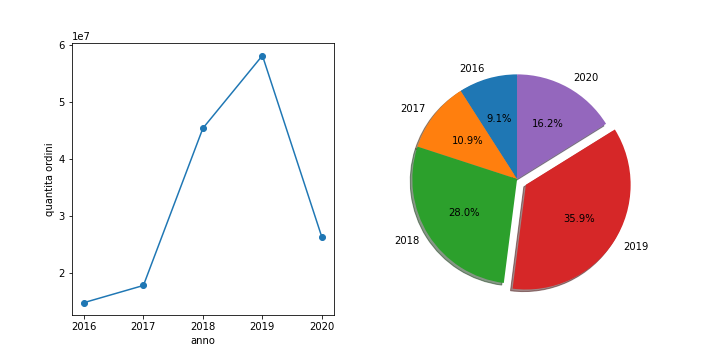
\includegraphics[scale=.5]{ordini_vs_anno.png}
\caption{Numero totale degli ordini per ogni anno.}
\label{ordi}
\end{figure}
dove bisogna sottolineare che i valori sull'ultimo anno (anno 2020) sono parziali poiché manca l'ultimo quadrimestre. 

In seguito, ho valutato i codici ordine con il maggior numero di ordini:
\begin{figure}[htb]
\centering
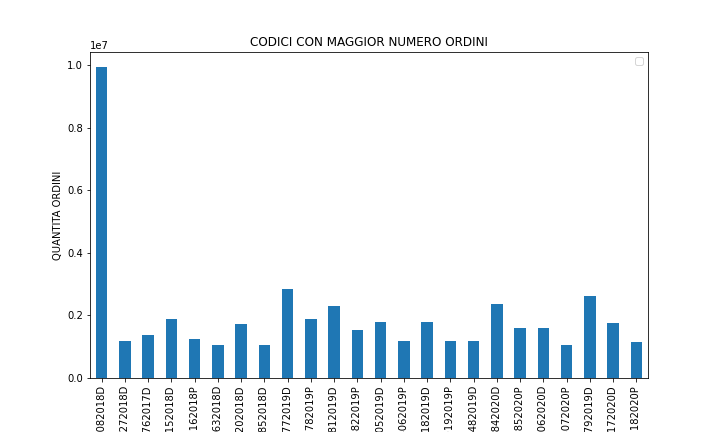
\includegraphics[scale=.5]{ordini_codici_hist.png}
\caption{Codici con maggior numero di ordini. Si considerano quantità non inferiori a un milione di pezzi.}
\label{pie}
\end{figure}
tuttavia, così visualizzati, i dati non aiutano a comprendere il trend. I codici, le cui cifre riportano caratteri alfanumerici presenti in altre colonne come ad esempio il valore di id dichiarazione, anno  e altro. Tuttavia tali codici non aiutano a comprendere il prodotto e perciò il grafico risulta di scarso impatto.

Ho trovato più utile valutare gli ordini in una base a una selezione delle categorie riportate. Infatti si trova che ogni codice è classificato in una delle 10 categorie (valori da 1 a 10) riportate nella colonna \textbf{a\_cod\_categoria}. 

\begin{figure}[htb]
\centering
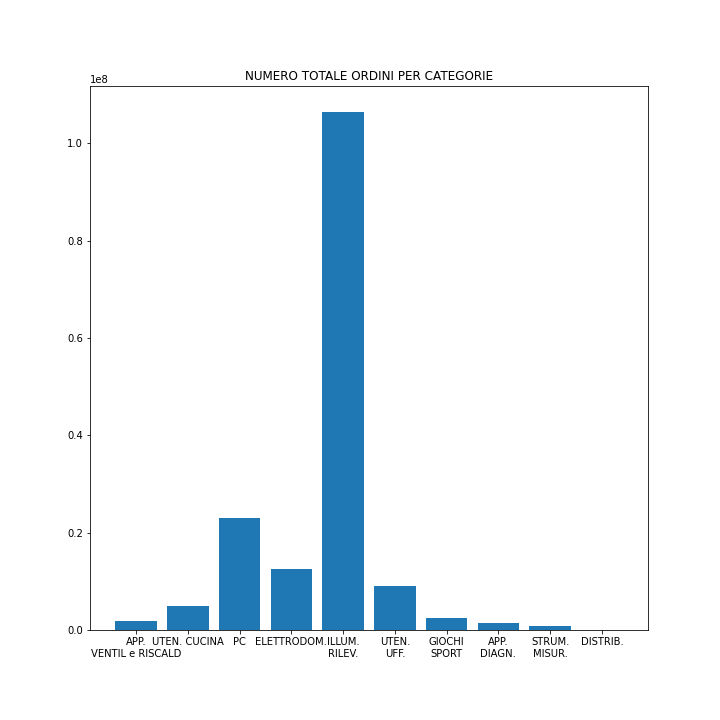
\includegraphics[scale=.5]{ordini_categorie_hist.png}
\caption{Numero totale degli ordini per ogni categoria.}
\label{hist}
\end{figure}

In fig.\ref{hist} viene riportata la quantità ordinata totale per ogni categoria.

Verificando le descrizioni riportate in colonna, si nota che alcuni prodotti a volte vengono inseriti in una categorie mentre in altre occasioni, dove la descrizione cambia di poco ma il prodotto descritto è lo stesso, la categoria selezionata è diversa.
Non mi pare chiaro quindi con quale logica vengono classificati i prodotti in una categoria rispetto ad un'altra.

\section*{Classificazione categoria del prodotto tramite la descrizione fornita}
La mia indagine parte dalla considerazione che descrizioni molto simili, a volte pressoché identiche (es. "apparecchi radio" si trova in categoria 4 e in categoria 5) sono inserite in categorie diverse. Ciò non è la situazione ideale qualora si volesse determinare le quantità vendute di un prodotto per ogni categoria, come riportato in fig.\ref{hist}. 
Considerando quindi che l'ordine di un prodotto può appartenere a categorie diverse anche se la descrizione riportata non cambia di molto, l'idea è di realizzare un classificatore che prende in input la descrizione, o meglio una lista di parole significative, chiamati \textbf{temi}, e attraverso un modello predittivo con le reti neurali assegna la descrizione ad una categoria con una certa probabilità. 
Per esempio, un classificatore in cui venga passato in input la frase \textit{computer con schermo} e presente nella categoria \textit{PC} può essere classificato, attraverso l'implementazione di un modello predittivo, nella categoria \textit{PC} oppure \textit{ELETTRODOMESTICI}, entrambi con una certa probabilità. 
Le categorie sono numerate dal valore 1 al 10: per semplicità assegnerò per convenzione un nome ad ognuna di esse anche se ciò non ha molto significato. Tale scelta ha solo un valore qualitativo per fare chiarezza. L'obiettivo ultimo del modello sarà quello di classificare descrizioni simili a una determinata categoria. Prima di ciò, sarà necessario verificare quanto il modello potrà essere affidabile nel suo giudizio. La valutazione del modello avverrà con i dati a disposizione, "istruendolo" con un set di training per poi metterlo alla prova con un set di test. 
In questa relazione verrà affrontato questo passaggio intermedio tramite l'utilizzo di questi due set di dati.

\subsection*{Impostazione problema}
Create le tabelle e inserite le descrizioni e le relative categorie, dobbiamo convertire tutte le descrizioni in un formato valido prima di poterle usare per istruire la rete neurale. Si effettueranno le seguenti operazioni:

\begin{itemize}
\item Creazione dei database attraverso uso di \textbf{SQLite} come sistema di gestione;
\item Estrazione delle parole significative (temi) all'interno della descrizione;
\item Costruzione di un classificatore attraverso l'uso di reti neurali artificiali.
\end{itemize}

\subsubsection*{Creazione del database}
Nella creazione dei database per le descrizioni e le categorie utilizzo \textbf{SQLite} come DBMS
\begin{verbatim}
categorie = """
    CREATE TABLE if not exists categorie(
    id INTEGER PRIMARY KEY AUTOINCREMENT, 
    categoria VARCHAR(50) NOT NULL);
"""

descrizioni = """
CREATE TABLE if not exists descrizioni(
       id INTEGER PRIMARY KEY AUTOINCREMENT,
       descrizione VARCHAR(255) NOT NULL,
       id_categoria INTEGER NOT NULL,
       
       FOREIGN KEY (id_categoria) REFERENCES categorie (id)
    );
"""
\end{verbatim}
ed eseguo le \textit{INSERT} prelevando le liste dei valori tramite il dataframe caricato con \textit{Pandas}. 

\subsubsection*{Ricavare parole significative della descrizione (temi)}
Per inserire le descrizioni è necessario eseguire un intervento preliminare.
In una descrizione prendiamo solo le parole significative che per semplicità indicheremo con il termine \textbf{temi}. Ciò sarà ottenuto tramite il modulo \textbf{stopwords} della libreria \textbf{nltk} il cui compito è quello di prelevare le parole poco significative all'interno di una frase.
Perciò si farà la seguente operazione di "pulizia" delle stringhe, partizionandole in un elenco di parole a cui verranno rimossi caratteri speciali e altre cose. 

In basso viene riportata la funzione creata per questo scopo specifico.
\begin{verbatim}
def bagOfWords(elem):
    """
    Partiziona la stringa in un elenco di parole.
    rimuove spazi, caratteri di punteggiatura,
    stop words, parole specifiche e caratteri speciali.
    Trasforma tutte le maiuscole in minuscole.
    """
    stringa = str(elem)
    words = stringa.lower().strip().split(' ')
    for word in words:
        word = word.rstrip().lstrip()
        if not re.match(':\/\/.*[\r\n]*', word) \
        and not re.match('^÷*[kg]', word) \
        and not re.match("\d", word) \
        and not re.match('^@.*""', word) \
        and re.match('^[a-z]', word) \
        and not re.match('\s', word) \
        and word not in stopwords:
            word = regex.sub("", word)
            if word:
                word.replace('"', '')
                yield word
\end{verbatim}

Ora che sappiamo eliminare da una frase le parole meno significative e le abbiamo inserite nel database creato, si implementa un metodo che elabori tutte le frasi del database. Dobbiamo creare tre liste:
\begin{enumerate}
\item La lista dei temi;
\item La lista delle categorie;
\item La lista dei documenti (ogni elemento è una tupla di due elementi: la lista dei temi e la categoria a cui appartiene);
\end{enumerate}

\begin{verbatim}
from nltk import word_tokenize

def elabora_corpus(corpus):
    """
    corpus sarà una lista di tuple, formata da:
    [
        ("una descrizione", "categoria1"),
        ("un'altra descrizione", "categoria2")
    ]
    """
    temi = set()
    categorie = set()
    documenti = []
    
    for descrizione, categoria in corpus:
   		parole = [
           	p.replace("'", '') for p in word_tokenize(descrizione)
          	if p not in stopwords
          	and p not in string.punctuation
        ]
        
        temi.update(descrizione)
        documenti.append((descrizione, categoria))
        categorie.add(categoria)
    
    temi = list(set(parola for parola in temi))
    categorie = list(categorie)

    return temi, categorie, documenti
\end{verbatim}
A questo metodo, daremo in ingresso i documenti ovvero le tuple (descrizioni "pulite", categoria) 
\begin{verbatim}
q = """
    SELECT  descrizione, categoria
    FROM descrizioni
    INNER JOIN categorie ON (id_categoria = categorie.id)
"""

documenti = cursor.execute(q).fetchall()

# elabora_corpus(<[(descrizione, categoria)]>)
temi, categorie, docs = elabora_corpus(documenti)
\end{verbatim}
A questo punto si avrà:
\begin{verbatim}
print("Numero categorie = {}".format(len(categorie))) --> Numero categorie = 10
print("Numero documenti = {}".format(len(docs))) --> Numero documenti = 18115
print('Numero temi = {}'.format(len(temi))) --> Numero temi = 402
print("Primi cinque temi = {}".format(temi[:5])) 
--> Primi cinque temi = ['centrale', 'videogiochi', 'indicare', 'dialisi', 'regolatori']
\end{verbatim}

\subsection*{Da un testo a un numero}

L'obiettivo sarà creare una lista per il training, ovvero delle casistiche per istruire la rete neurale. 
Per la rappresentazione numerica si considera la lista dei temi e quella delle categorie, ognuna di lunghezza pari alle liste originarie. La prima lista sarà l'input e la seconda l'output. I valori possibili degli elementi di queste due liste saranno due: 0 e 1. Verrà inserito il valore 1 nelle posizioni in cui un tema o una categoria sia contenuto. 

Per spiegare cosa si vuole ottenere, riporto un caso a titolo di esempio:
\begin{verbatim}

# Categorie osservate
categorie = ['DISTRIB.', 'APP.VENTIL. RISCALD.', 'APP. DIAGN.', 
'PC', 'GIOCHI SPORT', 'UTEN. CUCINA', 'ELETTRODOM.', 
'STRUM. MISUR.', 'UTEN. UFF.', 'ILLUM. RILEV.']

# Considero la lista di tuple documenti --> len(documenti) = 18115
# Ne prendo i primi due
print(documenti[:2]) -->
[("['asciugatrici']", 'APP.VENTIL. RISCALD.'), 
("['forni', 'microonde']", 'APP.VENTIL. RISCALD.')]

# Estraggo i TEMI_IN con metodo elabora_corpus()

TEMI_INT = ['asciugatrici', 'forni', 'microonde']

# Temi prelevati da tutti i documenti = TEMI_TOT -> len(TEMI_TOT) = 402

TEMI_TOT = [..., 'asciugatrici', ..., 'forni', ..., 'microonde']

X, y = crea_training_set(documenti[:2], categorie)

--> X = [..., [..., 1,..., 0,...],..., [..., 1,..., 1, ...,], ...]
--> y = [..., [0, 1, 0, 0, 0, 0, 0, 0, 0, 0], ... , [0, 1, 0, 0, 0, 0, 0, 0, 0, 0], ...]
--> len(X) = len(y) = 18115
\end{verbatim}
e lo useremo per creare il training set per la rete neurale, trasformando le frasi da un linguaggio naturale a uno numerico:

Per fare ciò si realizza il metodo seguente:
\begin{verbatim}
import random

def crea_training_set(documenti, categorie):
    """
    Metodo che ritorna una tupla di due valori:
        - l'array degli input (train_x)
        - l'array degli output (train_y)
        
    I due array hanno lungezza fissa:
     - len(train_x) == len(temi)
     - len(train_y) == len(categorie) 
    """
    training = []
    output_vuota = [0] * len(categorie)
    categorie = list(categorie)

    for parole, categoria in documenti:
        
        temi_descrizione = [parola for parola in parole]
        
        # riempio la lista di input
        riga_input = [1 if t in temi_descrizione else 0 for t in temi]

        # riempio la lista di output
        riga_output = output_vuota[:]
        riga_output[categorie.index(categoria)] = 1

        training.append([riga_input, riga_output])

    # mischio il mazzo
    random.shuffle(training)
    # trasformo in un array
    training = np.array(training)

    # e creo il training set
    train_x = list(training[:, 0])
    train_y = list(training[:, 1])
    return train_x, train_y
\end{verbatim}

\subsection*{Reti Neurali}
Viene proposta una rete neurale artificiale in cui gli strati di input ed output hanno numero di cerchi pari rispettivamente al numero di temi (402) e al numero di categorie (10). Il numero degli strati nascosti viene fissata a due mentre il numero di nodi all'interno sarà cambiato.

\subsubsection*{Schema generale}
\begin{figure}[p]
\centering
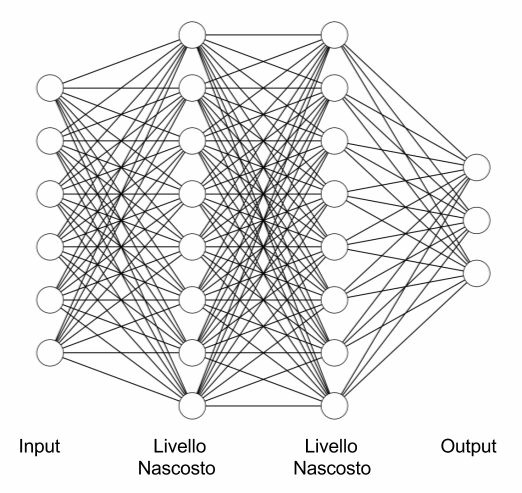
\includegraphics[scale=.6]{DNN}
\caption{Schema generale della rete neurale proposta.}
\label{deep}
\end{figure}

Ogni cerchio del diagramma in fig.~\ref{deep}, facente parte dei livelli esterni ed interni (nascosti), rappresenta un neurone (nodo). Ogni neurone è connesso agli altri neuroni dei livelli adiacenti. L'insieme di tutti i neuroni costituisce la rete neurale. Facendo un ingrandimento su ogni neurone, potremmo vederlo come in fig.~\ref{somme}

\begin{figure}[p]
\centering
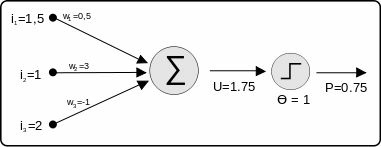
\includegraphics[scale=.6]{somme_neuroni}
\caption{Schema funzionamento singolo neurone.}
\label{somme}
\end{figure}

Anche qui, un ruolo importante lo giocano i pesi. In pratica, una rete neurale artificiale funziona così: si parte dai neuroni di input, ognuno dei quali codifica una feature del nostro dataset. Ogni neurone $i$ di input è connesso a ogni neurone $j$ del primo strato tramite una connessione identificata da un peso         $\omega_{ij}$. Gli input vengono dunque passati al primo strato della rete moltiplicati per il peso opportuno: il dato presente nel neurone 1 in input viene passato al neurone 7 dello strato successivo moltiplicato per il peso $\omega_{1,7}$, il dato nel neurone 2 in input viene passato al neurone 7 del primo strato moltiplicato per $\omega_{2,7}$ e così via. A questo punto il neurone 7 (ugualmente a tutti gli altri neuroni dello strato) somma tra loro tutti i segnali che gli arrivano e applica, al risultato, una funzione di attivazione : questo sarà l'output che dovrà trasmettere al secondo livello. Ugualmente a prima i neuroni del primo e del secondo livello sono connessi tra loro con dei pesi $\tilde{\omega}_{ij}$, quindi i gli output del primo livello vengono moltiplicati e sommati dai neuroni del secondo strato. L'algoritmo, come lo abbiamo appena descritto, prende il nome di \textbf{feedforward}.
La funzione di attivazione possiede due importarti proprietà:
\begin{itemize}
\item ha un valore di output compreso tra 0 e 1;
\item deve fornire un valore di output vicino ad 1 quando viene sufficientemente stimolata (in pratica deve simulare un effetto soglia), per propagare l'attività all'interno della rete.
\end{itemize}

Una delle funzioni matematiche utilizzate è la \textit{softmax}:
\begin{equation*}
softmax_i(a) = \frac{\exp a_i}{\Sigma\exp a_i}
\end{equation*}

La scelta di questa funzione è dovuta al tipo di classificazione poiché il modello dovrà classificare i dati scegliendo tra categorie differenti.
Di solito, nell'istruire una rete neurale, si parte assegnando dei pesi casuali a ciascun neurone. Con l'algoritmo feedforward, si calcola l'output per ogni input. Conoscendo l'output corretto che si vuole ottenere, si calcolano gli errori che questa rete commette e, con una tecnica simile a quella della regressione, si vanno ad aggiustare via via i valori dei pesi fino a ridurre al massimo i costi. La tecnica è simile a quella della regressione, ma non uguale, per due motivi: il primo è che si deve considerare la funzione di attivazione; il secondo è che i pesi del secondo strato si possono aggiustare guardando direttamente l'output, mentre quelli del primo strato si devono calibrare considerando l'errore che gli arriva "mediato" dal secondo livello. Questa tecnica è chiamata \textbf{backpropagation}.
La Rete Neurale che si vuole costruire sarà di tipo profondo (questo tipo di rete è anche conosciuto come Deep Neural Network, o DNN) e sarà composta da due livelli nascosti, ognuno contenente un numero variabile di neuroni. Teoricamente maggiore è il numero di neuroni, migliore è la resa del modello predittivo ma con un numero maggiore di esecuzioni dell'algoritmo sul set di training, chiamato con il termine \textbf{EPOCHS}. Il numero di \textbf{EPOCHS} può influenzare direttamente il risultato del training (con un numero esiguo di \textbf{EPOCHS} si può incorrere in un minimo locale). Per scrivere la rete neurale si farà uso della libreria di \textbf{Tensorflow}.

\subsubsection*{Funzionamento Deep Neural Network con Tensorflow}
La rete neurale da implementare per realizzare il classificatore sarà composta da un livello di input, due livelli nascosti, e uno di output. Come funzione di attivazione, verrà usata la funzione presentata \textit{softmax}. La realizzazione di una rete di questo tipo con \textbf{tflearn}, che sfrutta \textbf{Tensorflow}. Si utilizza con il codice seguente:

\begin{verbatim}
import tensorflow as tf
import tflearn
from tflearn import input_data, fully_connected, regression, DNN

def ClassificatoreANN(X, y):
    """
    Questo metodo definisce e istruisce una 
    ANN (Artificial Neural Network), di tipo
    DNN (Deep Neural Network) composta da:
        - un livello di input, 
        - due hidden layer,
        - uno di output.
    Utilizza softmax come funzione di attivazione.
    
    I parametri sono:
       - X: array bidimensionale con i dati di input
       - y: array bidimensionale con i dati di output
       
    Una volta definita la struttura della rete neurale,
    ne viene fatto il training, e il modello viene
    salvato in un file, chiamato "rete.tflearn".
    """
    
    # resetto i dati del grafo
    tf.compat.v1.reset_default_graph()
    
    # Definire la Rete Neurale
    rete = input_data(shape=[None, len(X[0])])
    rete = fully_connected(rete, HIDDEN_NODES)
    rete = fully_connected(rete, HIDDEN_NODES)
    rete = fully_connected(rete, len(y[0]), activation='softmax')
    rete = regression(rete)
    
    # Faccio il training
    model = DNN(rete, tensorboard_dir='logs', tensorboard_verbose=3)
    model.fit(X, y, n_epoch=EPOCHS, batch_size=8, show_metric=True)
    # Salvataggio modello
    model.save('Reti/rete_{}perc_ep{}_hid_{}'.format(PERC, EPOCHS, HIDDEN_NODES))
    return model

modello = ClassificatoreANN(X, y)
\end{verbatim}
Si realizzano i due set di dati che useremo per istruire il modello

\begin{verbatim}
# TRAINING SET con una percentuale PERC = 70% delle 18115 descrizioni
PERC = 70
nint = int(len(documenti)*int(PERC)/100)

TRAIN_SET = documenti[:nint]
TEST_SET = documenti[nint:]

X, y = crea_training_set(TRAIN_SET, categorie)
\end{verbatim}
selezionando il $70\%$ delle descrizioni che rappresenterà il training set. Il rimanente verrà utilizzato per i test finali del modello. 

Infine si può istruire la DNN del classificatore: 
\begin{verbatim}
modello = ClassificatoreANN(X, y)
modello.save('rete')
\end{verbatim}
e, una volta che l'esecuzione del calcolo del modello con il training set è terminata, la rete è istruita e i pesi dei vari neuroni sono stati salvati in file di testo.

Per verificare il funzionamento del modello si prende in input i documenti appartenenti al test set, attraverso il procedimento mostrato nella sezione precedente.
In seguito, tramite il metodo chiamato \textit{genera\_input}, si trasforma questa lista in valori numerici (in modo da avere un input scritto in un formato compatibile ad essere elaborato dalla rete definita).

\begin{verbatim}
# DA LISTA DI PAROLE a LISTA DI 0 e 1
def genera_input(lista_temi):
    """
    Conversione da lista di temi
    a lista di cifre costituita da 0 (no match) e 1 (match)
    """
    lista_input = [0]*len(temi) 
    for tema in lista_temi:
        for i, t in enumerate(temi):
            if t == tema: 
                lista_input[i] = 1
    return(np.array(lista_input))
\end{verbatim}
In modo che in output si possa avere un array (con lunghezza pari al numero dei temi) i cui valori sono 0 oppure 1 a seconda che il tema in ingresso siano presente tra quelli presi nel training set. 

\begin{verbatim}
SOGLIA_ERRORE = 0.25

def classifica(modello, array):
    # genera le probabilità da associare ad ognuna delle 10 categorie
    prob = modello.predict([array])[0] 
    # filtro quelle che superano la soglia di errore del 25%
    prob_d = {v: prob[i]  for i, v in enumerate(categorie)}
    risultati = [
        [i,p] for i,p in enumerate(prob) 
        if p > SOGLIA_ERRORE
    ]
    # ordino per le categorie più probabili in ordine decrescente
    risultati.sort(key=lambda x: x[1], reverse=True)
    lista_categorie = []
    for r in risultati:
        lista_categorie.append((list(categorie)[r[0]], r[1]))
    return lista_categorie
\end{verbatim}

ed infine implemento una funzione per selezionare le probabilità associate alle categorie predette.

\begin{verbatim}
def trova_categorie(modello, temi_descrizione):
    X = genera_input(temi_descrizione)
    # genero la classifica delle categorie predette (almeno con 25%)
    # inserendo i temi di input nel modello di rete neurale  
    categorie_predette = classifica(modello, X)
    
    if categorie_predette:
        # SELEZIONO CATEGORIE CON PROBABILITA' >= SOGLIA_ERRORE = 25%
        return categorie_predette
\end{verbatim}


\subsection*{Analisi predizione}

Vengono riportate le predizioni sui set di training e di test. I risultati saranno confrontati in base al numero di nodi negli strati interni, detti \textbf{HIDDEN NODES}, e il numero di campionamenti, chiamati \textbf{EPOCHS}.
Il calcolo è stato eseguito su un singolo pc, con un numero di \textbf{EPOCHS} non elevato. 

A livello preliminare, in basso sono mostrate tre predizioni eseguite sul training set:
\begin{verbatim}
cat_oss = []
cat_pred = []

for i, (desc_in, categoria_in) in enumerate(TRAIN_SET[:3]):
    print('\nTRAIN SET no. {}'.format(i+1))
    temi_test = estrai_temi(desc_in)
    print('\ncategoria osservata: {}'.format(categoria_in))
    cat_oss.append(categoria_in)
    c_pred = trova_categorie(modello, temi_test)
    cat_pred.append(c_pred[0][0])

TRAIN no. 1

categoria osservata: APP.VENTIL. RISCALD.

Le principali categorie (>=25%) predette sono 1 [(cat, prob)] --> 
[('APP.VENTIL. RISCALD.', 0.99999845)]

<-------------------------------->

TRAIN no. 2

categoria osservata: APP.VENTIL. RISCALD.

Le principali categorie (>=25%) predette sono 1 [(cat, prob)] --> 
[('APP.VENTIL. RISCALD.', 0.99999845)]

<-------------------------------->

TRAIN no. 3

categoria osservata: APP.VENTIL. RISCALD.

Le principali categorie (>=25%) predette sono 1 [(cat, prob)] --> 
[('APP.VENTIL. RISCALD.', 0.9999397)]

<-------------------------------->

Comparazione per le 3 categorie osservate vs predette [ True  True  True]
\end{verbatim}

Sommando i casi di \textit{match} (True) e \textit{non match} (False) tra categoria osservata e quella predetta nell'intero set di training (12680) e di set (5435), si ottengono i grafici in fig.\ref{h_64_100}.

\begin{figure}[htpb]
\centering
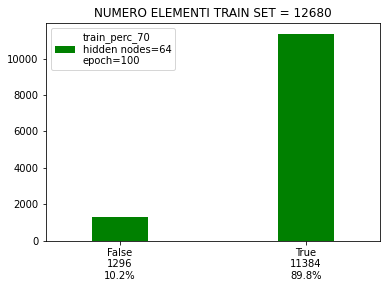
\includegraphics[scale=.6]{Plot/equality_train_perc_70_64_hidden_nodes_epoch_100.png}\\
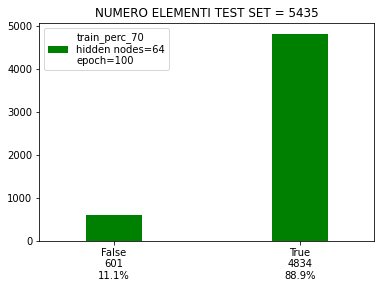
\includegraphics[scale=.6]{Plot/equality_test_perc_70_64_hidden_nodes_epoch_100.png}
\caption{Match tra categoria osservata vs predetta. \textbf{HIDDEN NODES} = 64, \textbf{EPOCHS} = 100.}
\label{h_64_100}
\end{figure}

%\begin{figure}[htpb]
%\centering
%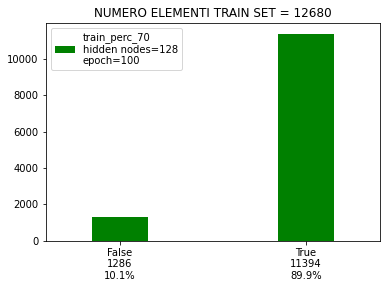
\includegraphics[scale=.6]{Plot/equality_train_perc_70_128_hidden_nodes_epoch_100.png}\\
%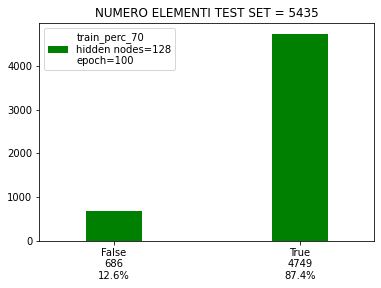
\includegraphics[scale=.6]{Plot/equality_test_perc_70_128_hidden_nodes_epoch_100.png}
%\caption{\textbf{HIDDEN NODES} = 128, \textbf{EPOCHS} = 100}
%\label{h_128_100}
%\end{figure}
%
\newpage

L'accuratezza della previsione del modello, vale a dire la percentuale di \textit{match} in rapporto al numero dei dati nel set, è mostrato in fig.\ref{acc_train} e fig.\ref{acc_test}.

\begin{figure}[htb]
\centering
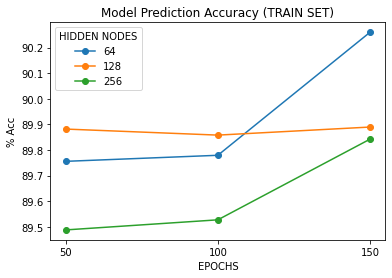
\includegraphics[scale=.6]{Plot/Accuracy_train_vs_epochs.png}
\caption{Accuratezza del modello vs \textbf{EPOCHS} utilizzando il training set. Il modello è stato testato con un diverso numero di \textbf{HIDDEN NODES}.}
\label{acc_train}
\end{figure}

\begin{figure}[htb]
\centering
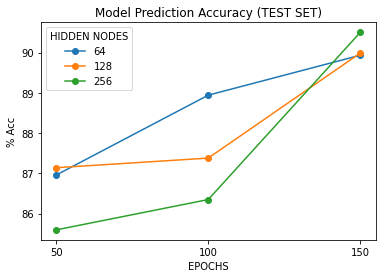
\includegraphics[scale=.6]{Plot/Accuracy_test_vs_epochs.png}
\caption{Accuratezza del modello vs \textbf{EPOCHS} utilizzando il test set. Il modello è stato testato con un diverso numero di \textbf{HIDDEN NODES}.}
\label{acc_test}
\end{figure}

La percentuale tra categorie predette ed osservate in entrambi i set è simile: ciò fa presumere che il numero di \textbf{EPOCHS} non è ancora sufficientemente alto. Infatti, a causa del numero limitato, si può intuire che la curva di errore (\textit{loss function}) in funzione degli \textbf{EPOCHS} non tende ancora a un valore di soglia minima e quindi l'accuratezza del metodo non è ottimale.

Idealmente per migliorare l'accuratezza del modello si dovrebbe considerare un numero alto di \textbf{HIDDEN NODES} e di \textbf{EPOCHS}. Tuttavia, a causa del numero limitato di \textbf{EPOCHS}, non sempre aumentare il numero di \textbf{HIDDEN NODES} si traduce in una migliore accuratezza, soprattutto quando il numero di dati in ingresso è elevato. 

Nel caso con \textbf{EPOCHS} = 150, il modello con \textbf{HIDDEN NODES} = 256 si dimostra più accurato solamente per il set di test (5435 dati) mentre nel set di training (12680 dati) ciò non vale.
In entrambi i set, diminuendo il numero di \textbf{EPOCHS}, non conviene considerare il modello con \textbf{HIDDEN NODES} = 256. 

\end{document}